% This file defines the command for plotting the ReLU function.
% It can be compiled standalone or included in a larger document.

\ifdefined\ispartofbook
\else
  % --- Standalone Compilation Preamble ---
  \documentclass[tikz, border=10pt]{standalone}
  \usepackage{tikz}
  \usetikzlibrary{arrows.meta}
  \begin{document}
\fi

% --- THE DIAGRAM COMMAND ---
\newcommand{\reluplot}{%
    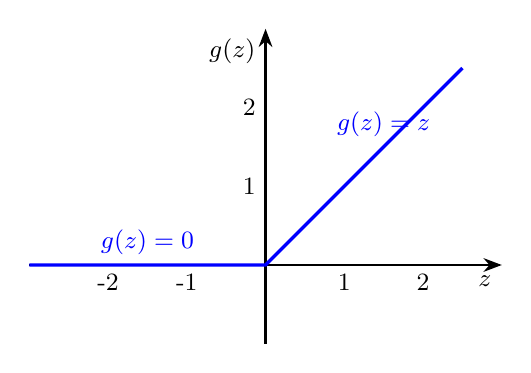
\begin{tikzpicture}[
        font=\sffamily,
        every node/.style={font=\small}
    ]
    % Axes
    \draw[-Stealth, thick] (-3,0) -- (3,0) node[below left] {$z$};
    \draw[-Stealth, thick] (0,-1) -- (0,3) node[below left] {$g(z)$};

    % Axis labels
    \node[below] at (-2, 0) {-2};
    \node[below] at (-1, 0) {-1};
    \node[below] at (1, 0) {1};
    \node[below] at (2, 0) {2};
    \node[left] at (0, 1) {1};
    \node[left] at (0, 2) {2};

    % ReLU function plot
    \draw[blue, very thick] (-3,0) -- (0,0) -- (2.5,2.5);

    % Annotations
    \node[above, blue] at (1.5, 1.5) {$g(z)=z$};
    \node[above, blue] at (-1.5, 0) {$g(z)=0$};
    
    \end{tikzpicture}%
}

\ifdefined\ispartofbook
  % This part is intentionally left blank when included in the main book.
  % The \newcommand is defined, and the chapter file is responsible for calling it.
\else
  % This part is for standalone compilation of the image.
  \reluplot
  \end{document}
\fi
